\documentclass[runningheads,a4paper]{llncs}

\usepackage[T1]{fontenc}
\usepackage[utf8]{inputenc}
\usepackage{microtype}
\usepackage{graphicx}
\usepackage{booktabs}
\usepackage{tabularx}
\usepackage{array}
\usepackage{amsmath}
\usepackage{amssymb}
\usepackage{mathtools}
\usepackage{threeparttable}
\usepackage{siunitx}
\usepackage{xcolor}
\usepackage{hyperref}

\newcolumntype{L}{>{\raggedright\arraybackslash}X}
\newcolumntype{C}{>{\centering\arraybackslash}X}

\graphicspath{{figures/}}
\hypersetup{
  colorlinks=true,
  linkcolor=blue!50!black,
  urlcolor=blue!50!black,
  citecolor=blue!50!black,
  pdftitle={Deep Re-annotation and Controlled Candidate Pools for Re-evaluating Ranking Models on MS MARCO},
  pdfauthor={, , and }
}

\setlength{\emergencystretch}{1.5em}
\setlength{\tabcolsep}{5pt}
\renewcommand{\arraystretch}{1.12}
\sisetup{
  detect-all,
  input-decimal-markers = {.},
  table-number-alignment = center
}

\title{Deep Re-annotation and Controlled Candidate Pools for Re-evaluating Ranking Models on MS MARCO}
\titlerunning{Deep Re-annotation and Controlled Candidate Pools}
\author{}
\authorrunning{}
\institute{}

\begin{document}

\maketitle
\begin{abstract}
This paper studies how additional manual relevance annotation changes the evaluation of retrieval models on MS MARCO, where the original annotation usually provides only one explicitly relevant passage per query. We analyze a manually annotated subset of 1,179 queries and 33,667 query-document pairs, comparing the original MS MARCO labels, extended human labels, and labels produced by a compact cross-encoder judge. Here, deep re-annotation means judging multiple candidate answers within a defined pool, rather than assuming that the original positive passage exhausts the relevant answers. The judge is then applied to a larger set of queries to study pseudo-relevance labels under controlled pooling depths. Manual re-annotation increases the average number of relevant documents per query from 1.07 to 17.47 and yields statistically significant gains in NDCG@10 for all considered ranking sources, for example from 0.597 to 0.877 for BM25 and from 0.701 to 0.967 for E5. On the full set, high pseudo-relevance density appears only after the judge is applied to a large pooled set built from the top BM25, E5, and BGE results. This value therefore cannot be interpreted without specifying the candidate pooling protocol.

\keywords{Information retrieval \and MS MARCO \and relevance judgments \and re-annotation \and pseudo-relevance labels \and pooling \and reciprocal rank fusion}
\end{abstract}

\section{Introduction}

Modern neural information retrieval systems require large collections of queries, documents, and relevance judgments. One of the most influential collections of this kind is MS MARCO, built from real Bing search queries and widely used for passage and document ranking \cite{bajaj2016msmarco}. The mMARCO dataset, its multilingual extension, includes Russian \cite{bonifacio2022mmarco}, and the Russian portion is used in RusBEIR, a benchmark for Russian information retrieval \cite{2025rusbeir}.

MS MARCO is one of several search-provider datasets, not a universal sample of information needs. Google's Natural Questions contains real search queries with human answer annotations on Wikipedia pages \cite{kwiatkowski2019naturalquestions}. Yahoo!'s Learning to Rank Challenge released two sets of query--document feature vectors and graded relevance labels without query or document text \cite{chapelle2011yahoo}. Yandex's Personalized Web Search Challenge released session and click logs with anonymized identifiers rather than readable queries and documents \cite{yandex2013personalized}. These are useful counterparts in search research, but their tasks and released representations differ from passage ranking.

We focus on MS MARCO because its accessible texts, sparse human judgments, established evaluation tools, and pretrained models support comparisons with prior work. The sparse judgments also provide a direct setting for studying additional annotation. This choice does not establish universality: provider-specific sampling, language, query intent, and document domain may affect transfer. Differences between countries or social groups are not measured in this study.

A central property of MS MARCO is the sparsity of its original relevance judgments. In the passage ranking task, most queries are associated with a single positive passage that may answer the user's question \cite{msmarco_datasets}. The standard file containing query-document relevance labels is commonly called qrels, short for query relevance judgments. This design is practical for large-scale training, but it can be incomplete for evaluation: other relevant passages may exist in the corpus but remain unjudged. A retrieval model may therefore return a useful document and still receive no credit because the document is absent from the qrels file.

This incompleteness matters especially when comparing systems of different types. Lexical methods such as BM25 rely on term matching \cite{robertson2009bm25}; dense retrievers such as E5 and BGE use separate vector representations of queries and documents \cite{wang2022e5,xiao2023cpack}; and cross-encoders score query-document pairs jointly \cite{nogueira2019bert}. These methods may retrieve different relevant documents. Re-evaluating MS MARCO after additional annotation is therefore not merely a matter of increasing absolute scores; it can also change the comparative picture between retrieval approaches.

By \emph{deep re-annotation} we mean extending relevance judgments across the candidate documents in a defined pool. ``Deep'' refers to annotation coverage, not neural-network depth or repeated training. It does not mean that the entire corpus has been exhaustively judged. For example, a query about why a liquid's boiling point increases may have several passages explaining the addition of salt. If only one passage is in the original qrels, another correct explanation receives zero gain until it is judged. Section~\ref{sec:example} gives an actual example with passage identifiers and before/after labels.

The retrieval rankings are held fixed when comparing original and human labels. Thus, an increase in measured NDCG after annotation does not mean that a retrieval model itself has improved. It means that its existing output is evaluated against more complete judgments. A second part of the study uses a learned judge to extend label coverage to larger candidate pools. These predictions are called \emph{pseudo-labels} to distinguish them from human judgments.

We study this problem at two levels. First, we analyze a manual subset for which additional human relevance judgments are available. This makes it possible to compare the original MS MARCO labels with denser human labels inside the same candidate pool. Second, we study a larger query set using a judge model: a binary classifier that receives a query-document pair and returns a relevance score. This judge is used because manually annotating the full set is impractical.

We also analyze Reciprocal Rank Fusion (RRF) \cite{cormack2009rrf}, a simple method for combining ranked lists. RRF assigns a higher score to documents that appear near the top of several input rankings. In this paper, RRF is used to test whether a simple fusion of retrieval lists improves the final ranking under the same relevance judgments.

The study addresses three research questions.
\begin{enumerate}
\item How does additional manual annotation change qrels density and retrieval quality metrics?
\item How reliable is a judge model as a tool for automatic pseudo-labeling?
\item How does pooling depth affect the number of pseudo-relevant documents and the quality of RRF-based fusion?
\end{enumerate}

By pooling depth we mean the number of top documents taken from each ranked list before merging. For example, at $K=10$ the judge receives the union of the top 10 documents from each system, while at $K=200$ it receives a much larger union. Thus, the density of pseudo-relevance labels in the full-set experiment is a property of the pooling protocol, not only of the corpus or the judge.

The main findings are as follows. Manual re-annotation significantly increases NDCG@10 for all ranking sources considered in the manual pool. The MiniLM-based cross-encoder judge \cite{wang2020minilm,reimers2019sentencebert} achieves sufficient held-out quality to serve as a reproducible baseline for pseudo-labeling. On the full query set, pseudo-qrels density is determined not only by corpus properties and judge quality, but also by the pooling protocol. Finally, RRF is useful only on a small controlled pool; its advantage disappears as the candidate pool expands.

\section{Related Work}

MS MARCO was introduced as a large-scale dataset based on real search queries and has become a standard testbed for text ranking \cite{bajaj2016msmarco}. The mMARCO dataset extends it through machine translation to several languages \cite{bonifacio2022mmarco}. For Russian, RusBEIR collects translated, adapted, and original Russian retrieval datasets for benchmark evaluation \cite{2025rusbeir}.

BM25 remains a standard lexical retrieval baseline, ranking documents through term frequency and document length normalization \cite{robertson2009bm25}. Dense retrieval methods represent queries and documents as vectors; widely used families include E5 \cite{wang2022e5} and BGE/FlagEmbedding \cite{xiao2023cpack}. Cross-encoders process a query and a document jointly and are commonly used for re-ranking candidate lists \cite{nogueira2019bert}.

Pooling is a standard approach for building information retrieval test collections: documents from the top ranks of several systems are merged and then judged by assessors \cite{voorhees2005trec}. Pooling reduces annotation cost, but it also makes the resulting qrels dependent on the systems and pool depth used to construct the pool.

Rank fusion is another related line of work. RRF was proposed as a simple way to combine ranked outputs from different retrieval systems without training additional parameters \cite{cormack2009rrf}. Later work on hybrid retrieval and retrieval-augmented generation has shown that RRF remains practically useful, but its effect depends on the input systems, list depth, and fusion parameters \cite{bruch2023fusion,mackenzie2023anserini,rackauckas2024ragfusion}.

Our work does not introduce a new retrieval model. Its contribution is a re-evaluation of existing ranking sources after additional annotation, an analysis of automatic pseudo-labeling with a judge model, and an explicit separation between judge quality and candidate-pool depth.

\section{Data, Pooling, and Manual Re-annotation}

\subsection{Source Collection}

The source material is MS MARCO Passage Ranking. It contains user queries, a corpus of 8,841,823 short passages, and qrels files, i.e., query relevance judgment files that specify documents considered relevant to the queries. The original development-set qrels contain 7,437 positive pairs for 6,980 queries. The manual subset contains 1,179 queries and 33,667 distinct query--passage pairs, with 28.56 candidates per query on average and a maximum of 63. The full-set candidate-pool protocol considered in this paper is larger: it uses 101,093 queries for which saved BM25, E5, and BGE rankings are available for pseudo-labeling.

The issue with the original labels is not that the positive documents are necessarily wrong, but that they often do not exhaust all acceptable answers in the corpus. If a query asks which county a place belongs to, the corpus may contain multiple passages that correctly state the same county. The original qrels may include only one of them. A system that retrieves another correct passage is then penalized because that passage is unjudged.

The manual pool was assembled by combining query-based retrieval results with auxiliary candidate-selection channels. Each query has ten entries in the saved BM25, E5, and BGE rankings. The annotation data also retain the auxiliary channels E5-rerank and E5-based similarity to a known relevant answer, as part of the reference-assisted annotation procedure. The similarity signal has access to answer information unavailable to ordinary query-only retrieval. They contribute candidates beyond the three query-only lists. In particular, 6,258 pairs have no score in BM25, E5, BGE, or E5-rerank; 35 pools contain more than 40 documents. Thus, the annotation pool includes additional candidates beyond the four named top-ten lists.

\subsection{Pooling Procedure}

To study missing judgments, we constructed a candidate pool for selected queries using pooling. The pool included top-ranked documents from BM25, a lexical retrieval baseline; E5 and BGE, dense bi-encoder retrievers; and an auxiliary E5-based signal that measures the similarity of a candidate to the known relevant answer for the same query. The last source is not an ordinary search model: unlike a deployed retrieval system, it uses the original MS MARCO relevant passage in addition to the query. We therefore use it only to expand the manual annotation pool, not as a full-set retrieval model.

For each query, the top 10 documents from each source were merged and duplicates were removed. Human assessors then judged the resulting query-document pairs. During annotation, the assessor saw the query, the candidate document, and the original relevant MS MARCO answer. This setup anchors the new judgments to the same interpretation of the information need as the original annotation.

\subsection{Dataset Characteristics}
\label{sec:example}

The manual subset contains 1,179 queries and 33,667 query-document pairs, with an average of 28.56 candidate documents per query. Inside this pool, the original MS MARCO qrels contain 1,257 positive pairs, or 1.07 relevant documents per query. After manual re-annotation, the number of positive pairs increases to 20,597, or 17.47 relevant documents per query. Thus, the new evaluation set does not replace MS MARCO; rather, it shows how strongly qrels density changes within a deliberately constructed pool.

\begin{table}[t]
\centering
\caption{Manual evaluation set before and after additional annotation.}
\label{tab:annotation-data}
\scriptsize
\setlength{\tabcolsep}{2pt}
\begin{tabularx}{\textwidth}{@{}>{\hsize=.85\hsize}L c c c c >{\hsize=1.15\hsize}L@{}}
\toprule
\textbf{Label set} & \textbf{Queries} & \textbf{Pairs} & \textbf{Positive} & \textbf{Rel./query} & \textbf{Comment} \\
\midrule
Original MS MARCO in the pool & 1179 & 33667 & 1257 & 1.07 & original relevant answers \\
Manual re-annotation & 1179 & 33667 & 20597 & 17.47 & original and newly found relevant documents \\
Judge labels on the same pool & 1179 & 33667 & 22193 & 18.82 & automatic labels after judge training \\
\bottomrule
\end{tabularx}
\end{table}

Table~\ref{tab:annotation-data} shows that the main effect of re-annotation is not an increase in the number of queries, but a sharp increase in the density of positive judgments within the candidate pool.

\begin{table}[t]
\centering
\caption{Pooled NDCG@10 on the manual subset before and after additional human annotation. Values are computed inside the annotated candidate pool and are not full-corpus leaderboard scores.}
\label{tab:main}
\footnotesize
\setlength{\tabcolsep}{4pt}
\begin{tabularx}{\textwidth}{@{}L c c c L@{}}
\toprule
\textbf{Ranking source} & \textbf{Original} & \textbf{Human} & \textbf{$\Delta$} & \textbf{Note} \\
\midrule
BM25 & 0.597 & 0.877 & +0.280 & lexical retrieval \\
E5 & 0.701 & 0.967 & +0.266 & dense retrieval from the query \\
BGE & 0.672 & 0.948 & +0.276 & dense retrieval from the query \\
E5 + seed answer & 0.708 & 0.975 & +0.267 & auxiliary pooling signal \\
RRF & 0.607 & 0.906 & +0.299 & rank fusion \\
\bottomrule
\end{tabularx}
\end{table}

Table~\ref{tab:main} shows that additional annotation changes both qrels density and measured ranking quality. The auxiliary ``E5 + seed answer'' signal has the highest value on the manual pool, as expected, because it uses the original relevant document. It should therefore not be interpreted as a deployable retrieval system.

\paragraph{Example.}
For query 1086224, ``what causes boiling point to increase'', Table~\ref{tab:annotation-example} contrasts an original relevant passage, an additional relevant answer, and a negative candidate. The descriptions are shortened paraphrases of the stored passages.

\begin{table}[t]
\centering
\caption{A concrete annotation example. ``Unjudged'' means absent from the original positive qrels, not necessarily irrelevant.}
\label{tab:annotation-example}
\small
\begin{tabularx}{\textwidth}{@{}l L l l@{}}
\toprule
Passage ID & Passage content & Original & Human \\
\midrule
7112148 & Adding salt to water increases its boiling point. & Relevant & Relevant \\
7399382 & Adding a non-volatile solute, such as salt, raises a solvent's boiling point. & Unjudged & Relevant \\
987600 & Reports the boiling temperature of acetone. & Unjudged & Not relevant \\
\bottomrule
\end{tabularx}
\end{table}

A system returning passage 7399382 receives no gain for that passage under the original sparse qrels. After the additional human judgment, the same passage contributes positive gain without any change to the system's ranking.


\section{Task Formulation and Experimental Protocol}

Let $\mathcal{Q}$ be a set of queries, $\mathcal{D}$ the document corpus, and $\mathcal{M}$ a set of ranking systems. For a query $q \in \mathcal{Q}$ and a system $m \in \mathcal{M}$, let $\mathrm{TopK}_m(q)$ denote the set of the first $K$ documents in the ranking returned by $m$. The pooled candidate set is
\begin{equation}
\label{eq:pool}
P_q^{(K)} = \bigcup_{m \in \mathcal{M}} \mathrm{TopK}_m(q).
\end{equation}

The parameter $K$ controls the pooling depth. At $K=10$, the first 10 documents from each system are used; at $K=200$, the first 200 documents from each system are used. After merging and duplicate removal, the pool may contain fewer than $K \cdot |\mathcal{M}|$ documents.

In the manual subset, we evaluate four ranking sources inside the pool: BM25 as a lexical baseline, E5 and BGE as dense bi-encoder retrievers, and the auxiliary ``E5 + seed answer'' signal. The first three sources use only the query and can therefore be applied to the larger query set. The fourth source uses the original relevant MS MARCO answer and is used only for manual pooling.

\subsection{Judge Model}

The judge model is introduced to transfer the manual annotation signal to candidate pools that are too large to annotate exhaustively by humans. It is not used as an additional retrieval system and does not replace BM25, E5, or BGE. Those systems generate candidate documents; the judge assigns binary pseudo-relevance labels to already selected query-document pairs. Therefore, the judge is evaluated as a pairwise relevance classifier rather than as a first-stage retriever on the original qrels.

The judge is a cross-encoder: the query and the candidate passage are processed jointly by the transformer. This differs from E5 and BGE, which are bi-encoder retrievers that encode queries and documents separately and compare their vector representations. A cross-encoder is slower, but it can model token-level interactions between the query and the candidate document and is therefore commonly used for pairwise relevance assessment.

The judge model is based on \texttt{cross-encoder/ms-marco-MiniLM-L-6-v2}, a compact MiniLM-based cross-encoder distributed through the Sentence-Transformers model collection \cite{wang2020minilm,reimers2019sentencebert}.\footnote{\url{https://huggingface.co/cross-encoder/ms-marco-MiniLM-L-6-v2}} We use it because it is public, reproducible, already trained for MS MARCO passage ranking, and computationally feasible for a controlled re-annotation study. The unmodified base model reaches ROC-AUC 0.865 on our validation split; after fine-tuning on the manual labels, validation ROC-AUC increases to 0.908. The judge receives only the text of the query and the text of the candidate document. Embeddings, ranks, and scores from BM25, E5, BGE, or RRF are not passed to the judge; these systems are used only for candidate generation and subsequent comparison.

The judge was fine-tuned on the manual subset of 1,179 queries and 33,667 pairs. The split was performed by query identifiers in a 70/15/15 proportion with random seed 42: 23,543 pairs from 825 queries for training, 5,122 pairs from 177 queries for validation, and 5,002 pairs from 177 queries for testing. All documents of the same query were assigned to the same split. The binarization threshold was selected on the validation part and equals $\tau=-0.2187$.

Let $s_\theta(q,d)$ be the judge score for the query-document pair and let $\tau$ be the binarization threshold. The judge decision is
\begin{equation}
\label{eq:judge}
\hat y_{\theta,\tau}(q,d) = \mathbb{I}\left[s_\theta(q,d) \ge \tau\right].
\end{equation}

The corresponding set of pseudo-relevant documents in the pool is
\begin{equation}
\label{eq:positive-set}
R_q^{(K)} = \left\{ d \in P_q^{(K)} \; \middle| \; \hat y_{\theta,\tau}(q,d) = 1 \right\},
\end{equation}
and the positive-label density is
\begin{equation}
\label{eq:density}
\rho_q^{(K)} = \frac{|R_q^{(K)}|}{|P_q^{(K)}|}.
\end{equation}

\subsection{Full-set Protocol}

For the larger query set, we use saved BM25, E5, and BGE ranked lists. For each pooling depth $K \in \{10,30,50,100,200\}$, the top $K$ results from each system are merged into the pooled set \eqref{eq:pool}. The judge then scores all query-document pairs in this pool and produces pseudo-qrels by applying the threshold $\tau$. Thus, the full-set results depend not only on judge quality, but also on how many candidates are presented to it.

\begin{figure}[t]
\centering
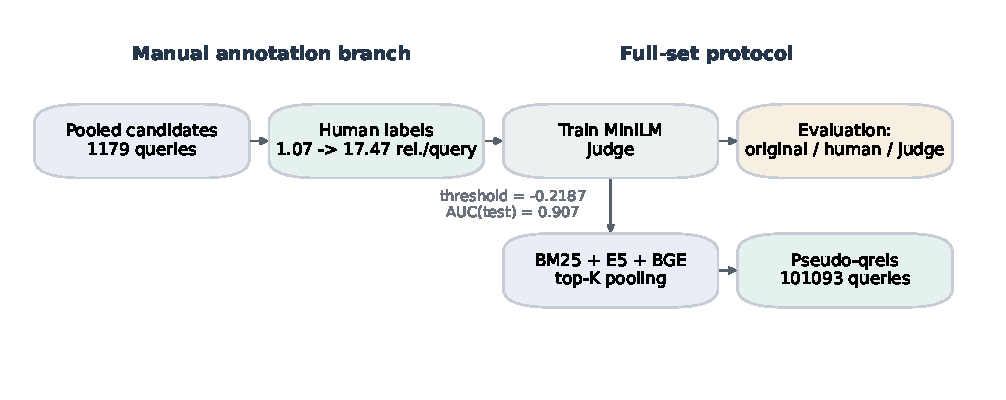
\includegraphics[width=0.92\textwidth]{protocol_schematic_en.pdf}
\caption{Experimental protocol. The upper branch corresponds to manual re-annotation and judge training. The lower branch corresponds to the full-set pseudo-labeling protocol with controlled pooling depth.}
\label{fig:protocol}
\end{figure}

Figure~\ref{fig:protocol} highlights the difference between the manual and full-set settings. The manual subset increases qrels density inside a relatively small pool. In the full-set setting, the judge receives much larger pools, so high pseudo-qrels density cannot be interpreted without the value of $K$.

\section{Metrics and Significance Testing}

The main ranking metric is NDCG@10, normalized discounted cumulative gain at the first ten retrieved positions. For a query $q$,
\begin{align}
\label{eq:dcg}
\mathrm{DCG}@10(q) &= \sum_{i=1}^{10} \frac{2^{\mathrm{rel}_i(q)} - 1}{\log_2(i + 1)}, \\
\label{eq:ndcg}
\mathrm{NDCG}@10(q) &= \frac{\mathrm{DCG}@10(q)}{\mathrm{IDCG}@10(q)}.
\end{align}

RRF is computed as
\begin{equation}
\label{eq:rrf}
\mathrm{RRF}(d \mid q) = \sum_{m \in \mathcal{M}} \frac{1}{c + \mathrm{rank}_m(d,q)}, \qquad c = 60.
\end{equation}

Pairwise comparisons are performed at the query level using a paired permutation test. For systems $A$ and $B$, define
\begin{equation}
\label{eq:delta}
\Delta_q = \mathrm{NDCG}_A(q) - \mathrm{NDCG}_B(q),
\end{equation}
with observed statistic
\begin{equation}
\label{eq:perm}
T = \frac{1}{|\mathcal{Q}'|} \sum_{q \in \mathcal{Q}'} \Delta_q,
\end{equation}
where $\mathcal{Q}'$ is the set of queries for which both systems have valid scores. In the permutation test, the signs of $\Delta_q$ are randomly flipped, and the $p$-value is estimated as the fraction of permutations whose absolute statistic is at least as large as the observed one.

\section{Results of Manual Re-annotation}

\subsection{Qrels Density Shift}

The first central result is that deep re-annotation substantially changes qrels density. On the manual subset, the average number of relevant documents per query increases from 1.07 to 17.47, and the median increases from 1 to 17.5. For judge labels on the same manual pool, the median increases further to 19. On the full pseudo-labeled set, the median reaches 93 and the 99th percentile reaches 401.

The value of about 130 pseudo-relevant documents per query should not be read as a direct estimate of the corpus' true relevance density. It appears in the full protocol at $K=200$, where the average pool size is 451.54 documents per query. The observed density is therefore a joint consequence of judge behavior and candidate presentation.

\subsection{Ranking Quality Change}

Manual re-annotation significantly increases NDCG@10 for all ranking sources in the manual pool. This includes lexical retrieval, dense retrieval, the seed-answer auxiliary signal, and RRF. Judge-based labels on the manual pool further increase the metric values, but those values must be interpreted separately from human labels because they include judge errors.

\begin{figure}[t]
\centering
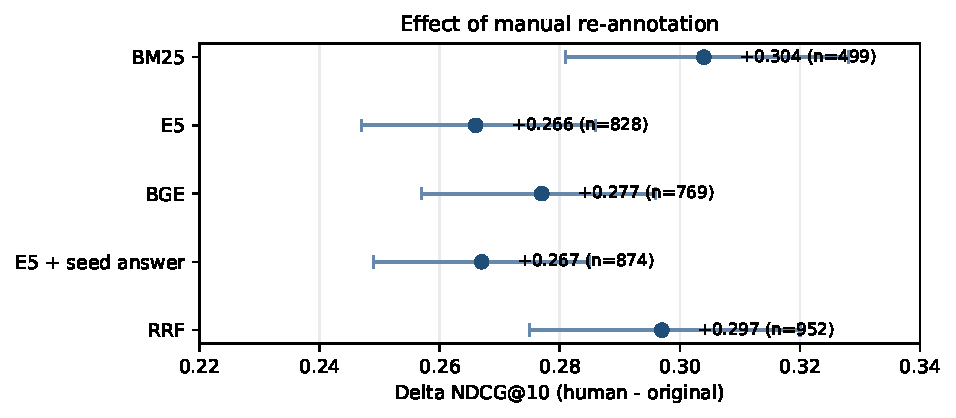
\includegraphics[width=\columnwidth]{manual_effect_forest_en.pdf}
\caption{Effect sizes for the transition from original labels to additional human labels. Points show mean paired NDCG@10 gains; intervals are 95\% bootstrap confidence intervals.}
\label{fig:effect-forest}
\end{figure}

\begin{table}[t]
\centering
\caption{Paired effect estimates for the transition from original labels to additional human labels.}
\label{tab:effect-ci}
\footnotesize
\begin{tabularx}{\columnwidth}{Lccc}
\toprule
\textbf{Ranking source} & \textbf{$\Delta$NDCG@10} & \textbf{95\% CI} & \textbf{Queries} \\
\midrule
BM25 & +0.304 & [0.281; 0.328] & 499 \\
E5 & +0.266 & [0.247; 0.286] & 828 \\
BGE & +0.277 & [0.257; 0.296] & 769 \\
E5 + seed answer & +0.267 & [0.249; 0.285] & 874 \\
RRF & +0.297 & [0.275; 0.320] & 952 \\
\bottomrule
\end{tabularx}
\end{table}

Tables~\ref{tab:main} and \ref{tab:effect-ci}, together with Fig.~\ref{fig:effect-forest}, show that the increase is systematic. All listed paired permutation tests produce $p < 0.001$, and the bootstrap confidence intervals do not cross zero.

RRF is not the best configuration on the manual subset. Under human labels, the seed-answer signal reaches 0.975, whereas RRF reaches 0.906. This is expected because the seed-answer signal uses the original relevant answer and therefore has access to information unavailable to ordinary retrieval systems.

\subsection{Judge Quality}

The MiniLM judge is not intended as the strongest possible relevance model; it is a reproducible baseline for automatic relevance assessment. On held-out data, it reaches ROC-AUC 0.908 on validation and 0.907 on test, with test F1 0.875 and Cohen's $\kappa=0.636$. It covers 95.05\% of manually relevant pairs and has 87.97\% precision against human labels.

\begin{figure}[t]
\centering
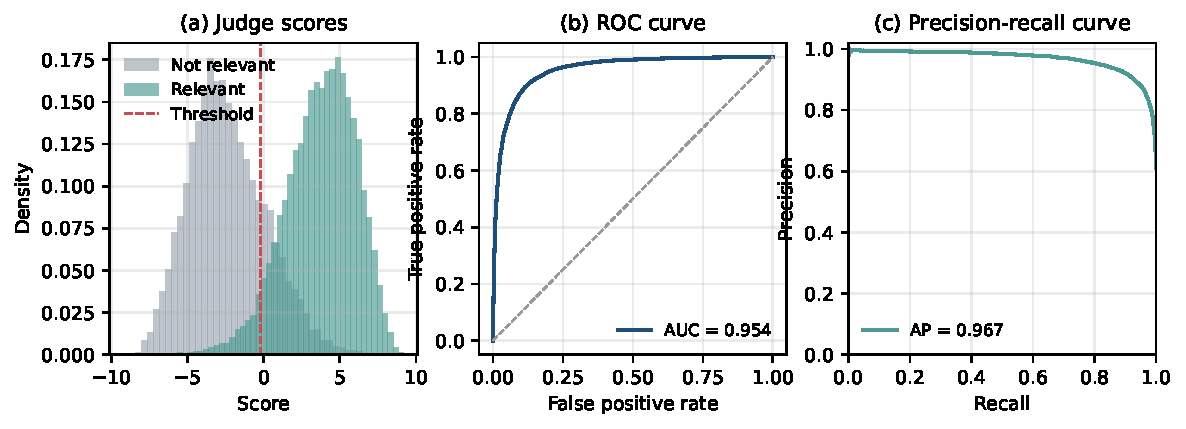
\includegraphics[width=0.95\textwidth]{judge_score_diagnostics_en.pdf}
\caption{Judge-score diagnostics on the annotated manual pool: score distributions, ROC curve, and precision-recall curve.}
\label{fig:judge}
\end{figure}

Figure~\ref{fig:judge} shows that relevant and non-relevant pairs are well separated at the score level. This supports the use of the judge as a baseline pseudo-labeling tool, while leaving room for future comparisons with stronger cross-encoders.

\begin{figure}[t]
\centering
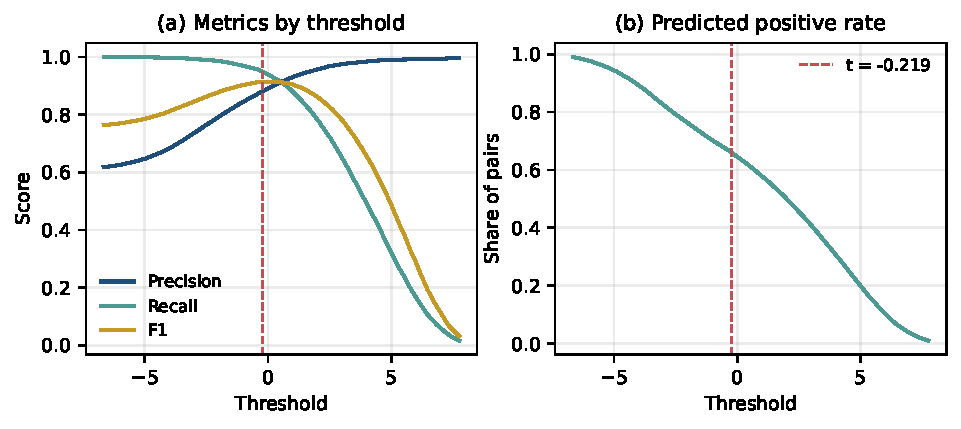
\includegraphics[width=0.90\textwidth]{judge_threshold_sensitivity_en.pdf}
\caption{Sensitivity of judge decisions to the threshold $\tau$. The vertical line marks the selected working threshold $\tau=-0.2187$.}
\label{fig:judge-threshold}
\end{figure}

At the selected threshold, the annotated manual pool has precision 0.881, recall 0.949, F1 0.914, and predicted-positive share 0.660. These values describe the operating point on the annotated pool; they should not be confused with held-out generalization metrics.

\section{Full-set Pseudo-qrels and Controlled Pooling}

The full-set protocol shows that pseudo-qrels must be analyzed together with pooling depth. At $K=10$, the average number of candidates per query is 21.88 and the average number of pseudo-relevant documents is 14.19. At $K=200$, these values increase to 451.54 and 128.64, respectively, while the positive-label share decreases from 0.649 to 0.285.

\begin{figure}[t]
\centering
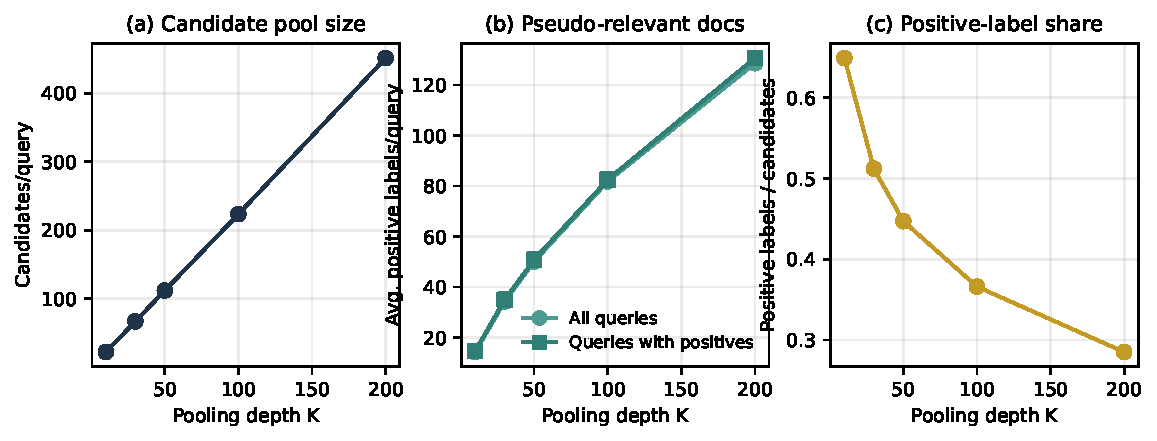
\includegraphics[width=0.94\textwidth]{pool_scaling_multipanel_en.pdf}
\caption{Pseudo-qrels properties under increasing full-set pooling depth. The number of pseudo-relevant documents must be interpreted together with the number of candidates shown to the judge.}
\label{fig:pool-scaling}
\end{figure}

\begin{figure}[t]
\centering
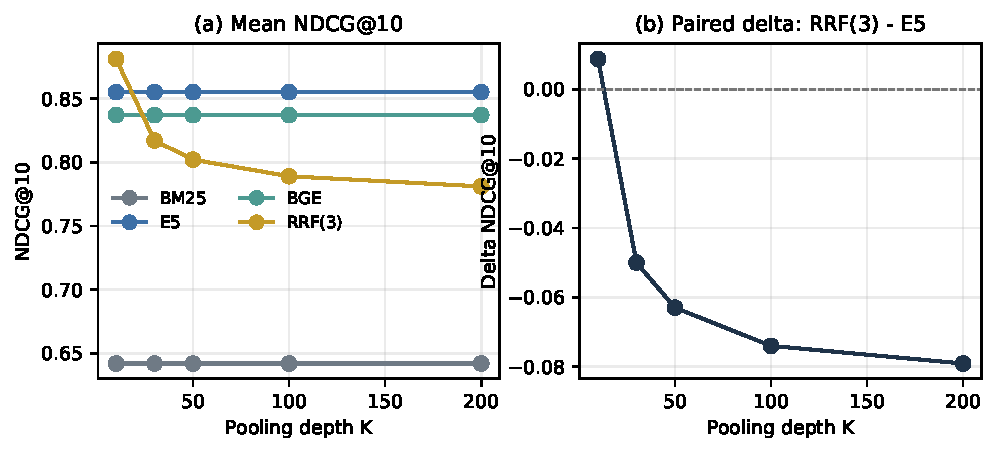
\includegraphics[width=0.94\textwidth]{fullset_uncertainty_panels_en.pdf}
\caption{Full-set ranking behavior under controlled pooling depth. Left: mean NDCG@10 for BM25, E5, BGE, and RRF(3). Right: paired $\Delta$NDCG@10 between RRF(3) and E5.}
\label{fig:fullset-uncertainty}
\end{figure}

Figures~\ref{fig:pool-scaling} and \ref{fig:fullset-uncertainty} summarize the main full-set result. At the narrow pool $K=10$, RRF has the best mean value among the available full-set configurations: 0.881 compared with 0.855 for E5 and 0.837 for BGE. As $K$ increases, RRF monotonically decreases: 0.817 at $K=30$, 0.802 at $K=50$, 0.789 at $K=100$, and 0.781 at $K=200$. The paired ``RRF minus E5'' difference is positive only at $K=10$ ($\Delta=+0.0087$, 95\% CI [0.0075; 0.0098]) and becomes negative from $K=30$ onward.

\begin{table}[t]
\centering
\caption{Key paired comparisons supporting the main conclusions.}
\label{tab:sig}
\scriptsize
\setlength{\tabcolsep}{3pt}
\begin{tabularx}{\columnwidth}{@{}L c c c@{}}
\toprule
\textbf{Comparison} & \textbf{$\Delta$ NDCG@10} & \textbf{$p$-value} & \textbf{Queries} \\
\midrule
RRF vs BM25 under human labels & +0.0372 & $< 0.001$ & 1102 \\
RRF vs E5 under human labels & -0.0582 & $< 0.001$ & 1171 \\
RRF vs E5 + seed answer under human labels & -0.0680 & $< 0.001$ & 1175 \\
RRF at $K=10$ vs E5 & +0.0087 & $< 0.001$ & 95517 \\
RRF at $K=200$ vs E5 & -0.0791 & $< 0.001$ & 98527 \\
\bottomrule
\end{tabularx}
\end{table}

Table~\ref{tab:sig} confirms two linked conclusions. First, on human labels RRF is below the seed-answer-assisted signal. Second, on full-set pseudo-qrels, the sign of RRF's advantage over E5 changes when moving from $K=10$ to $K=200$. Claims about the strength of rank fusion therefore cannot be transferred between protocols without specifying the pool.

\section{Threats to Validity and Discussion}

\paragraph{Construct validity.}
Deep re-annotation changes both metric values and system comparisons. Sparse MS MARCO qrels can underestimate strong dense retrievers and fusion methods. At the same time, both human and pseudo labels depend on which documents were presented for judgment.

\paragraph{Protocol validity.}
High-density pseudo-qrels on the full set cannot be discussed independently of pooling depth. The value of roughly 130 positive judgments per query is a property of the specific full-set protocol, not a natural constant of MS MARCO.

\paragraph{Judge validity.}
The judge analysis combines held-out classification metrics with score diagnostics on the annotated pool. These pieces of evidence are complementary but not identical. ROC and precision-recall diagnostics describe the operating behavior of the judge, whereas validation/test AUC and F1 describe generalization to held-out queries.

The selected MiniLM cross-encoder should be read as a reproducible baseline rather than as the strongest possible judge. More recent or larger rerankers, including BGE cross-encoder variants, may produce different pseudo-qrels and should be compared in a separate controlled experiment. Another natural extension is a relevance-answer-conditioned judge that receives the known relevant MS MARCO passage together with the candidate document, because the manual-pooling results show that similarity to the seed answer is a strong signal. We do not use such a signal in the full-set protocol, since using a known relevant document at evaluation time would give the judge external answer information that is unavailable to an ordinary query-only retrieval system.

\paragraph{External validity.}
The full-set part is limited to BM25, E5, and BGE, because these systems produce query-only rankings. The seed-answer signal is used only for manual pooling and is not a deployable full-corpus retrieval system. All conclusions are specific to MS MARCO and to the candidate selection protocol studied here.

\paragraph{Practical implications.}
The results answer the three research questions. First, manual re-annotation significantly increases NDCG@10 and qrels density. Second, the MiniLM judge is a usable baseline for pseudo-labeling, but its threshold and held-out quality must be controlled. Third, the interpretation of the 130.7 figure is inseparable from pooling depth, and RRF is useful only under a small controlled pool.

\section{Conclusion}

This paper shows that deep re-annotation on MS MARCO substantially changes qrels density and significantly increases NDCG@10 for all ranking sources considered in the manual pool. On this pool, the highest score is achieved by an auxiliary signal that uses the original relevant answer, while E5 remains the best ordinary query-only retrieval system. The MiniLM judge provides a reproducible baseline for automatic pseudo-labeling.

The full-set experiment deliberately uses a strict query-only setting for automatic pseudo-labeling: the judge receives a query and a candidate document, but not the original relevant MS MARCO passage. This restriction keeps the protocol comparable to ordinary retrieval outputs and avoids giving the judge external answer information that ordinary retrieval systems do not have. At the same time, the manual-pooling results show that the known relevant answer is a strong signal. A natural direction for future work is therefore to study a relevance-answer-conditioned judge with the input format ``query, known relevant answer, candidate document under assessment'', and to compare it with stronger cross-encoder models.

For the full-set protocol, pooling depth is a key factor in interpreting the results. With a small pool, RRF is the best available configuration, but its quality decreases monotonically as the pool expands. Pseudo-qrels density and fusion gains should therefore be analyzed together with the candidate selection protocol.

In practical terms, full-corpus pseudo-labeling is useful as a research instrument, but it requires controlled candidate pools and explicit restrictions when conclusions are stated. Thus, re-evaluating MS MARCO should be discussed not only as improving relevance judgments, but also as refining the evaluation protocol itself.

\section*{Acknowledgements}



\begin{thebibliography}{99}

\bibitem{bajaj2016msmarco}
P.~Bajaj, D.~Campos, N.~Craswell, L.~Deng, J.~Gao, X.~Liu, R.~Majumder, A.~McNamara, B.~Mitra, T.~Nguyen, M.~Rosenberg, X.~Song, A.~Stoica, S.~Tiwary, T.~Wang.
\newblock \textit{MS MARCO: A Human Generated MAchine Reading COmprehension Dataset}.
\newblock arXiv preprint arXiv:1611.09268, 2016.

\bibitem{bonifacio2022mmarco}
L.~Bonifacio, V.~Jeronymo, H.~Queiroz Abonizio, I.~Campiotti, M.~Fadaee, R.~Lotufo, R.~Nogueira.
\newblock \textit{mMARCO: A Multilingual Version of MS MARCO Passage Ranking Dataset}.
\newblock arXiv preprint arXiv:2108.13897, 2021.

\bibitem{2025rusbeir}
G.~, M.~Tikhomirov, E.~Kozhevnikov, M.~Kornilov, N.~.
\newblock \textit{Building Russian Benchmark for Evaluation of Information Retrieval Models}.
\newblock Computational Linguistics and Intellectual Technologies, 2025.

\bibitem{kwiatkowski2019naturalquestions}
T.~Kwiatkowski, J.~Palomaki, O.~Redfield, et al.
\newblock \textit{Natural Questions: A Benchmark for Question Answering Research}.
\newblock Transactions of the Association for Computational Linguistics, 7, 2019.
\newblock \url{https://doi.org/10.1162/tacl_a_00276}.

\bibitem{chapelle2011yahoo}
O.~Chapelle, Y.~Chang.
\newblock \textit{Yahoo! Learning to Rank Challenge Overview}.
\newblock Proceedings of the Learning to Rank Challenge, PMLR 14:1--24, 2011.
\newblock \url{https://proceedings.mlr.press/v14/chapelle11a.html}.

\bibitem{yandex2013personalized}
Yandex.
\newblock \textit{Personalized Web Search Challenge}.
\newblock Kaggle competition, 2013--2014.
\newblock \url{https://www.kaggle.com/c/yandex-personalized-web-search-challenge}, accessed 2026.


\bibitem{msmarco_datasets}
Microsoft.
\newblock \textit{MS MARCO datasets}.
\newblock \url{https://microsoft.github.io/msmarco/}, accessed 2026.

\bibitem{robertson2009bm25}
S.~E. Robertson, H.~Zaragoza.
\newblock \textit{The Probabilistic Relevance Framework: BM25 and Beyond}.
\newblock Foundations and Trends in Information Retrieval, 3(4):333--389, 2009.

\bibitem{wang2022e5}
L.~Wang, N.~Yang, X.~Huang, B.~Jiao, L.~Yang, D.~Jiang, R.~Majumder, F.~Wei.
\newblock \textit{Text Embeddings by Weakly-Supervised Contrastive Pre-training}.
\newblock arXiv preprint arXiv:2212.03533, 2022.

\bibitem{xiao2023cpack}
S.~Xiao, Z.~Liu, P.~Zhang, N.~Muennighoff, D.~Lian, J.-Y. Nie.
\newblock \textit{C-Pack: Packed Resources for General Chinese Embeddings}.
\newblock arXiv preprint arXiv:2309.07597, 2023.

\bibitem{nogueira2019bert}
R.~Nogueira, K.~Cho.
\newblock \textit{Passage Re-ranking with BERT}.
\newblock arXiv preprint arXiv:1901.04085, 2019.

\bibitem{cormack2009rrf}
G.~V. Cormack, C.~L.~A. Clarke, S.~B{\"u}ttcher.
\newblock \textit{Reciprocal Rank Fusion outperforms Condorcet and Individual Rank Learning Methods}.
\newblock In \textit{Proceedings of the 32nd Annual International ACM SIGIR Conference on Research and Development in Information Retrieval}, pp.~758--759, 2009.

\bibitem{wang2020minilm}
W.~Wang, F.~Wei, L.~Dong, H.~Bao, N.~Yang, M.~Zhou.
\newblock \textit{MiniLM: Deep Self-Attention Distillation for Task-Agnostic Compression of Pre-Trained Transformers}.
\newblock Advances in Neural Information Processing Systems, 33:5776--5788, 2020.

\bibitem{reimers2019sentencebert}
N.~Reimers, I.~Gurevych.
\newblock \textit{Sentence-BERT: Sentence Embeddings using Siamese BERT-Networks}.
\newblock In \textit{Proceedings of EMNLP-IJCNLP}, pp.~3982--3992, 2019.

\bibitem{voorhees2005trec}
E.~M. Voorhees, D.~K. Harman.
\newblock \textit{TREC: Experiment and Evaluation in Information Retrieval}.
\newblock MIT Press, 2005.

\bibitem{bruch2023fusion}
S.~Bruch, S.~Gai, A.~Ingber.
\newblock \textit{An Analysis of Fusion Functions for Hybrid Retrieval}.
\newblock arXiv preprint arXiv:2210.11934, 2022.

\bibitem{mackenzie2023anserini}
X.~Ma, T.~Teofili, J.~Lin.
\newblock \textit{Anserini Gets Dense Retrieval: Integration of Lucene's HNSW Indexes}.
\newblock In \textit{Proceedings of the 32nd ACM International Conference on Information and Knowledge Management}, 2023.

\bibitem{rackauckas2024ragfusion}
Z.~Rackauckas.
\newblock \textit{RAG-Fusion: A New Take on Retrieval-Augmented Generation}.
\newblock International Journal on Natural Language Computing, 13(1), 2024.

\end{thebibliography}

\clearpage
\section*{Reviewers' Remarks and Authors' Responses}
\noindent Submission 90. DAMDID 2026.

\paragraph{Reviewer 1: explanation and examples.}
\emph{Remark, summarized and translated from Russian.} The paper contains the necessary research sections, but the meaning of deep re-annotation is unclear. The reviewer finds the English presentation difficult to follow and requests concrete examples to explain the main concepts.

\emph{Response.} The Abstract and Introduction now define deep re-annotation as extending judgments over multiple candidate answers in a selected pool. The definition distinguishes annotation coverage from neural-network depth and from exhaustive annotation of the corpus. The Introduction also explains that denser judgments change the evaluation of fixed rankings, rather than improve the retrieval model itself. Section~\ref{sec:example} and Table~\ref{tab:annotation-example} provide a real MS MARCO query, passage identifiers, shortened passage descriptions, and before/after labels. The example shows why an unjudged correct answer receives no credit under sparse qrels.

\paragraph{Reviewer 2: overall assessment.}
\emph{Remark, summarized.} The reviewer considers the dataset-improvement problem important, the results valuable, and the strategy justified, and supports publication as a full paper.

\emph{Response.} We thank the reviewer for this assessment. No specific additional change was requested.

\paragraph{Reviewer 3: other providers and universality.}
\emph{Remark, summarized.} Are counterparts of MS MARCO available from Google, Yandex, or Yahoo? How universal is MS MARCO given differences in search-engine use between countries and social groups? The reviewer suggests explaining the choice of MS MARCO in the Introduction.

\emph{Response.} Two paragraphs have been added to the Introduction. They discuss Google's Natural Questions, Yahoo!'s Learning to Rank Challenge, and Yandex's Personalized Web Search Challenge with references to their source publications or dataset pages. The text distinguishes text-based question answering, ranking feature vectors, and anonymized interaction logs, rather than treating these resources as interchangeable passage-ranking datasets. MS MARCO is motivated by accessible texts, sparse judgments, established evaluation tools, and pretrained models. The Introduction explicitly states that differences between countries or social groups were not measured and that the collection is not a universal sample of information needs.


\end{document}
